

%\newcommand*{\ACM}{}%

\ifdefined\ACM

%\documentclass[sigplan,screen]{acmart}
  \documentclass[manuscript,screen,review]{acmart}

\else
  \documentclass{article}
  \usepackage[utf8]{inputenc}
\usepackage[a4paper, total={6in, 9in}]{geometry}
\usepackage{braket}
\usepackage{xcolor}
\usepackage{amsmath}
\usepackage{amsfonts}
\usepackage{amsthm}
\usepackage{amssymb}
%\usepackage[ocgcolorlinks]{hyperref}
\usepackage{hyperref}
%\usepackage{hyperref,xcolor}
%\usepackage[ocgcolorlinks]{ocgx2}
\usepackage{cleveref}
\usepackage{graphicx}
\usepackage{svg}
\usepackage{float}
\usepackage{tikz}
\usetikzlibrary{patterns, shapes.arrows}
\usepackage{adjustbox}
%\usepackage{tikz-network}
\usepackage{tkz-graph}
\usepackage{tkz-berge}
\usepackage[linesnumbered]{algorithm2e}
\usepackage{multicol}
\usepackage[backend=biber,style=alphabetic,sorting=ynt]{biblatex}
%\usepackage{xcolor}
%\usepackage{tkz-berge}
%\usepackage{tkz-graph}
\usepackage{pgfplots}
\usepackage{sagetex}
\usepackage{setspace}
\usepackage{etoc}
%\usepackage{wrapfig}
\usepackage{pgfgantt}
\DeclareUnicodeCharacter{2212}{−}
\usepgfplotslibrary{groupplots,dateplot}
\pgfplotsset{compat=newest}

\newtheorem{theorem}{Theorem}
\newtheorem{definition}{Definition}
\newtheorem{example}{Example}
\newtheorem{claim}{Claim}
\newtheorem{fact}{Fact}
\newtheorem{remark}{Remark}
\newtheorem*{theorem*}{Theorem}
\newtheorem{lemma}{Lemma}
\crefname{lemma}{Lemma}{Lemmas}
\hypersetup{colorlinks=true}
% , allcolors=blue,allbordercolors=blue,pdfborderstyle={0 0 1}}
%\hypersetup{pdfborder={2 2 2}}
% pdfpagemode=FullScreen,
% backref 

\newtheorem{problem}{Problem}
\crefname{problem}{Problem}{Problems}

\DeclareMathOperator{\Ima}{Im}


  \addbibresource{./sample.bib} 

\fi

\begin{document}

\newcommand{\commentt}[1]{\textcolor{blue}{ \textbf{[COMMENT]} #1}}
\newcommand{\ctt}[1]{\commentt{#1}}
\newcommand{\prb}[1]{ \mathbf{Pr} \left[ #1 \right]}
\newcommand{\prbm}[2]{ \mathbf{Pr}_{ #2 }\left[ #1 \right]}
\newcommand{\prbc}[3]{ \mathbf{Pr}_{ #2 }\left[ #1 \right | #3]}
\newcommand{\prbcprb}[3]{ \prbc{#2}{#1}{#3} \cdot \prb{#3} } 
\newcommand{\expp}[1]{ \mathbf{E} \left[ {#1} \right]}
\newcommand{\onotation}[1]{\(\mathcal{O} \left( {#1}  \right) \)}
\newcommand{\ona}[1]{\onotation{#1}}
\newcommand{\PSI}{{\ket{\psi}}}
\newcommand{\xij} { X_{ij} } 
\DeclareMathOperator{\Ima}{Im}
%\newcommand{\LESn}{\ket{\psi_n}}
%\newcommand{\LESa}{\ket{\phi_n}}
%\newcommand{\LESs}{\frac{1}{\sqrt{n}}\sum_{i}{\ket{\left(0^{i}10^{n-i}\right)^{n}}}}
%\newcommand{\Hn}{\mathcal{H}_{n}}
%\newcommand{\Ep}{\frac{1}{\sqrt{2^n}}\sum^{2^n}_{x}{ \ket{xx}}}
%\newcommand{\HON}{\ket{\psi_{\text{honest}}}}
%\newcommand{\Lemma}{\paragraph{Lemma.}}
\newcommand{\Cpa}{[n, \rho n, \delta n]}
%\setlength{\columnsep}{0.6cm}
\newcommand{\Jvv}{ \bar{J_{v}} } 
\newcommand{\Cvv}{ \tilde{C_{v}} } 

\newcommand{\Gz}{ G_{z}^{\delta} } 
\newcommand{ \Tann } {  \mathcal{T}\left( G, C_0 \right) }
\newcommand{\ireducable}{ireducable \hyperref[ire]{[\ref{ire}]} }
\newcommand{\cutUU}{E(U_{-1} \bigcup U_{+1} ,U)} 
\newcommand{\wcutUU}{w\left( E(U_{-1} \bigcup U_{+1} ,U)  \right)}
\newcommand{\testgo}{  \mathcal{T}\left(J, q , C_{0}\right) } 

\newcommand{\duC}{\left( C_{A}^{\perp}\otimes C_{B}^{\perp} \right)^{\perp}}
\newcommand{\duduC}{\left( C_{A}\otimes C_{B}\right)^{\perp}}
  





\title{Generate States.} 
\author{David Ponarovsky}
%\author{Noa Viner, David Ponarovsky}

\ifdefined\ACM
  \affiliation{%
    \institution{The Th{\o}rv{\"a}ld Group}
    \streetaddress{1 Th{\o}rv{\"a}ld Circle}
    \city{Hekla}
  \country{Iceland}}
  \email{larst@affiliation.org}
\else
  \maketitle
\fi
%
\abstract{We propose an alternative simple construction of good LTC codes. In contrast to previews, constructions made by \cite{Dinur}, \cite{leverrier2022quantum} and \cite{Pavel}, our construction doesn't require spicel properties of the small codes, such as $w$-robustness and $p$-resistance for puncturing.  
} 


\ifdefined\ACM
  \maketitle
\fi

%\begin{multicols*}{2}
% \section{Preambles}

Localy Testable Codes, or LTC, are error correction codes such that verfining a uinformly random cchoosen check, would be enough to detect any error with probability proportional to it's size. Bisdes the clear computional adventage they offer, they took roles at the eriler PCP proofs.  
  In this work, we propose a new construction for good LTC codes, which also have a good testability parameter. In the sense   Our proof also indirectly answers the following question. Why most of the good LDPC codes are known to be bad in terms of detecting errors? In other words, It seems that for most of them, there exist strings that are very far from being in the code and, meanwhile, fail to satisfy only a small number of restrictions.
  While the previous LDPC constructions focused on ensuring that the yielded code would have a good rate and distance parameters, our construction enforces the restrictions collection to have a nontrivial fraction of degeneration. That is, removing a single restriction will not change the code, as any restriction is linearly dependent on the others.






\begin{problem} Given amplitudes $\{ a_{i} \}_{0}^{2^{n}}$ Show that there is a Quantum cuircuit that generate $\ket{\psi} = \sum_{i}{a_{i}\ket{i}}$.
\end{problem}

\section{Control Gate.}
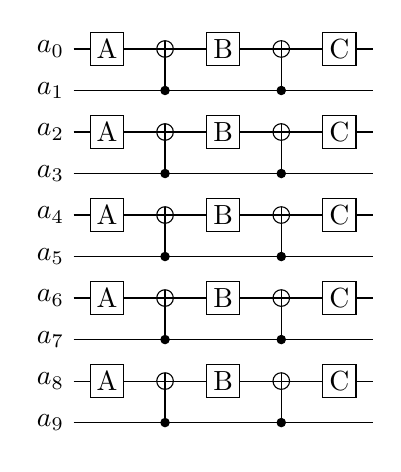
\begin{tikzpicture}[scale=1.000000,x=1pt,y=1pt]
\filldraw[color=white] (0.000000, -7.500000) rectangle (108.000000, 142.500000);
% Drawing wires
% Line 1: a0 W a_0
\draw[color=black] (0.000000,135.000000) -- (108.000000,135.000000);
\draw[color=black] (0.000000,135.000000) node[left] {$a_0$};
% Line 2: a1 W a_1
\draw[color=black] (0.000000,120.000000) -- (108.000000,120.000000);
\draw[color=black] (0.000000,120.000000) node[left] {$a_1$};
% Line 3: a2 W a_2
\draw[color=black] (0.000000,105.000000) -- (108.000000,105.000000);
\draw[color=black] (0.000000,105.000000) node[left] {$a_2$};
% Line 4: a3 W a_3
\draw[color=black] (0.000000,90.000000) -- (108.000000,90.000000);
\draw[color=black] (0.000000,90.000000) node[left] {$a_3$};
% Line 5: a4 W a_4
\draw[color=black] (0.000000,75.000000) -- (108.000000,75.000000);
\draw[color=black] (0.000000,75.000000) node[left] {$a_4$};
% Line 6: a5 W a_5
\draw[color=black] (0.000000,60.000000) -- (108.000000,60.000000);
\draw[color=black] (0.000000,60.000000) node[left] {$a_5$};
% Line 7: a6 W a_6
\draw[color=black] (0.000000,45.000000) -- (108.000000,45.000000);
\draw[color=black] (0.000000,45.000000) node[left] {$a_6$};
% Line 8: a7 W a_7
\draw[color=black] (0.000000,30.000000) -- (108.000000,30.000000);
\draw[color=black] (0.000000,30.000000) node[left] {$a_7$};
% Line 9: a8 W a_8
\draw[color=black] (0.000000,15.000000) -- (108.000000,15.000000);
\draw[color=black] (0.000000,15.000000) node[left] {$a_8$};
% Line 10: a9 W a_9
\draw[color=black] (0.000000,0.000000) -- (108.000000,0.000000);
\draw[color=black] (0.000000,0.000000) node[left] {$a_9$};
% Done with wires; drawing gates
% Line 11: a0 G A
\begin{scope}
\draw[fill=white] (12.000000, 135.000000) +(-45.000000:8.485281pt and 8.485281pt) -- +(45.000000:8.485281pt and 8.485281pt) -- +(135.000000:8.485281pt and 8.485281pt) -- +(225.000000:8.485281pt and 8.485281pt) -- cycle;
\clip (12.000000, 135.000000) +(-45.000000:8.485281pt and 8.485281pt) -- +(45.000000:8.485281pt and 8.485281pt) -- +(135.000000:8.485281pt and 8.485281pt) -- +(225.000000:8.485281pt and 8.485281pt) -- cycle;
\draw (12.000000, 135.000000) node {A};
\end{scope}
% Line 16: a2 G A
\begin{scope}
\draw[fill=white] (12.000000, 105.000000) +(-45.000000:8.485281pt and 8.485281pt) -- +(45.000000:8.485281pt and 8.485281pt) -- +(135.000000:8.485281pt and 8.485281pt) -- +(225.000000:8.485281pt and 8.485281pt) -- cycle;
\clip (12.000000, 105.000000) +(-45.000000:8.485281pt and 8.485281pt) -- +(45.000000:8.485281pt and 8.485281pt) -- +(135.000000:8.485281pt and 8.485281pt) -- +(225.000000:8.485281pt and 8.485281pt) -- cycle;
\draw (12.000000, 105.000000) node {A};
\end{scope}
% Line 21: a4 G A
\begin{scope}
\draw[fill=white] (12.000000, 75.000000) +(-45.000000:8.485281pt and 8.485281pt) -- +(45.000000:8.485281pt and 8.485281pt) -- +(135.000000:8.485281pt and 8.485281pt) -- +(225.000000:8.485281pt and 8.485281pt) -- cycle;
\clip (12.000000, 75.000000) +(-45.000000:8.485281pt and 8.485281pt) -- +(45.000000:8.485281pt and 8.485281pt) -- +(135.000000:8.485281pt and 8.485281pt) -- +(225.000000:8.485281pt and 8.485281pt) -- cycle;
\draw (12.000000, 75.000000) node {A};
\end{scope}
% Line 26: a6 G A
\begin{scope}
\draw[fill=white] (12.000000, 45.000000) +(-45.000000:8.485281pt and 8.485281pt) -- +(45.000000:8.485281pt and 8.485281pt) -- +(135.000000:8.485281pt and 8.485281pt) -- +(225.000000:8.485281pt and 8.485281pt) -- cycle;
\clip (12.000000, 45.000000) +(-45.000000:8.485281pt and 8.485281pt) -- +(45.000000:8.485281pt and 8.485281pt) -- +(135.000000:8.485281pt and 8.485281pt) -- +(225.000000:8.485281pt and 8.485281pt) -- cycle;
\draw (12.000000, 45.000000) node {A};
\end{scope}
% Line 31: a8 G A
\begin{scope}
\draw[fill=white] (12.000000, 15.000000) +(-45.000000:8.485281pt and 8.485281pt) -- +(45.000000:8.485281pt and 8.485281pt) -- +(135.000000:8.485281pt and 8.485281pt) -- +(225.000000:8.485281pt and 8.485281pt) -- cycle;
\clip (12.000000, 15.000000) +(-45.000000:8.485281pt and 8.485281pt) -- +(45.000000:8.485281pt and 8.485281pt) -- +(135.000000:8.485281pt and 8.485281pt) -- +(225.000000:8.485281pt and 8.485281pt) -- cycle;
\draw (12.000000, 15.000000) node {A};
\end{scope}
% Line 12: +a0 a1
\draw (33.000000,135.000000) -- (33.000000,120.000000);
\begin{scope}
\draw[fill=white] (33.000000, 135.000000) circle(3.000000pt);
\clip (33.000000, 135.000000) circle(3.000000pt);
\draw (30.000000, 135.000000) -- (36.000000, 135.000000);
\draw (33.000000, 132.000000) -- (33.000000, 138.000000);
\end{scope}
\filldraw (33.000000, 120.000000) circle(1.500000pt);
% Line 17: +a2 a3
\draw (33.000000,105.000000) -- (33.000000,90.000000);
\begin{scope}
\draw[fill=white] (33.000000, 105.000000) circle(3.000000pt);
\clip (33.000000, 105.000000) circle(3.000000pt);
\draw (30.000000, 105.000000) -- (36.000000, 105.000000);
\draw (33.000000, 102.000000) -- (33.000000, 108.000000);
\end{scope}
\filldraw (33.000000, 90.000000) circle(1.500000pt);
% Line 22: +a4 a5
\draw (33.000000,75.000000) -- (33.000000,60.000000);
\begin{scope}
\draw[fill=white] (33.000000, 75.000000) circle(3.000000pt);
\clip (33.000000, 75.000000) circle(3.000000pt);
\draw (30.000000, 75.000000) -- (36.000000, 75.000000);
\draw (33.000000, 72.000000) -- (33.000000, 78.000000);
\end{scope}
\filldraw (33.000000, 60.000000) circle(1.500000pt);
% Line 27: +a6 a7
\draw (33.000000,45.000000) -- (33.000000,30.000000);
\begin{scope}
\draw[fill=white] (33.000000, 45.000000) circle(3.000000pt);
\clip (33.000000, 45.000000) circle(3.000000pt);
\draw (30.000000, 45.000000) -- (36.000000, 45.000000);
\draw (33.000000, 42.000000) -- (33.000000, 48.000000);
\end{scope}
\filldraw (33.000000, 30.000000) circle(1.500000pt);
% Line 32: +a8 a9
\draw (33.000000,15.000000) -- (33.000000,0.000000);
\begin{scope}
\draw[fill=white] (33.000000, 15.000000) circle(3.000000pt);
\clip (33.000000, 15.000000) circle(3.000000pt);
\draw (30.000000, 15.000000) -- (36.000000, 15.000000);
\draw (33.000000, 12.000000) -- (33.000000, 18.000000);
\end{scope}
\filldraw (33.000000, 0.000000) circle(1.500000pt);
% Line 13: a0 G B
\begin{scope}
\draw[fill=white] (54.000000, 135.000000) +(-45.000000:8.485281pt and 8.485281pt) -- +(45.000000:8.485281pt and 8.485281pt) -- +(135.000000:8.485281pt and 8.485281pt) -- +(225.000000:8.485281pt and 8.485281pt) -- cycle;
\clip (54.000000, 135.000000) +(-45.000000:8.485281pt and 8.485281pt) -- +(45.000000:8.485281pt and 8.485281pt) -- +(135.000000:8.485281pt and 8.485281pt) -- +(225.000000:8.485281pt and 8.485281pt) -- cycle;
\draw (54.000000, 135.000000) node {B};
\end{scope}
% Line 18: a2 G B
\begin{scope}
\draw[fill=white] (54.000000, 105.000000) +(-45.000000:8.485281pt and 8.485281pt) -- +(45.000000:8.485281pt and 8.485281pt) -- +(135.000000:8.485281pt and 8.485281pt) -- +(225.000000:8.485281pt and 8.485281pt) -- cycle;
\clip (54.000000, 105.000000) +(-45.000000:8.485281pt and 8.485281pt) -- +(45.000000:8.485281pt and 8.485281pt) -- +(135.000000:8.485281pt and 8.485281pt) -- +(225.000000:8.485281pt and 8.485281pt) -- cycle;
\draw (54.000000, 105.000000) node {B};
\end{scope}
% Line 23: a4 G B
\begin{scope}
\draw[fill=white] (54.000000, 75.000000) +(-45.000000:8.485281pt and 8.485281pt) -- +(45.000000:8.485281pt and 8.485281pt) -- +(135.000000:8.485281pt and 8.485281pt) -- +(225.000000:8.485281pt and 8.485281pt) -- cycle;
\clip (54.000000, 75.000000) +(-45.000000:8.485281pt and 8.485281pt) -- +(45.000000:8.485281pt and 8.485281pt) -- +(135.000000:8.485281pt and 8.485281pt) -- +(225.000000:8.485281pt and 8.485281pt) -- cycle;
\draw (54.000000, 75.000000) node {B};
\end{scope}
% Line 28: a6 G B
\begin{scope}
\draw[fill=white] (54.000000, 45.000000) +(-45.000000:8.485281pt and 8.485281pt) -- +(45.000000:8.485281pt and 8.485281pt) -- +(135.000000:8.485281pt and 8.485281pt) -- +(225.000000:8.485281pt and 8.485281pt) -- cycle;
\clip (54.000000, 45.000000) +(-45.000000:8.485281pt and 8.485281pt) -- +(45.000000:8.485281pt and 8.485281pt) -- +(135.000000:8.485281pt and 8.485281pt) -- +(225.000000:8.485281pt and 8.485281pt) -- cycle;
\draw (54.000000, 45.000000) node {B};
\end{scope}
% Line 33: a8 G B
\begin{scope}
\draw[fill=white] (54.000000, 15.000000) +(-45.000000:8.485281pt and 8.485281pt) -- +(45.000000:8.485281pt and 8.485281pt) -- +(135.000000:8.485281pt and 8.485281pt) -- +(225.000000:8.485281pt and 8.485281pt) -- cycle;
\clip (54.000000, 15.000000) +(-45.000000:8.485281pt and 8.485281pt) -- +(45.000000:8.485281pt and 8.485281pt) -- +(135.000000:8.485281pt and 8.485281pt) -- +(225.000000:8.485281pt and 8.485281pt) -- cycle;
\draw (54.000000, 15.000000) node {B};
\end{scope}
% Line 14: +a0 a1
\draw (75.000000,135.000000) -- (75.000000,120.000000);
\begin{scope}
\draw[fill=white] (75.000000, 135.000000) circle(3.000000pt);
\clip (75.000000, 135.000000) circle(3.000000pt);
\draw (72.000000, 135.000000) -- (78.000000, 135.000000);
\draw (75.000000, 132.000000) -- (75.000000, 138.000000);
\end{scope}
\filldraw (75.000000, 120.000000) circle(1.500000pt);
% Line 19: +a2 a3
\draw (75.000000,105.000000) -- (75.000000,90.000000);
\begin{scope}
\draw[fill=white] (75.000000, 105.000000) circle(3.000000pt);
\clip (75.000000, 105.000000) circle(3.000000pt);
\draw (72.000000, 105.000000) -- (78.000000, 105.000000);
\draw (75.000000, 102.000000) -- (75.000000, 108.000000);
\end{scope}
\filldraw (75.000000, 90.000000) circle(1.500000pt);
% Line 24: +a4 a5
\draw (75.000000,75.000000) -- (75.000000,60.000000);
\begin{scope}
\draw[fill=white] (75.000000, 75.000000) circle(3.000000pt);
\clip (75.000000, 75.000000) circle(3.000000pt);
\draw (72.000000, 75.000000) -- (78.000000, 75.000000);
\draw (75.000000, 72.000000) -- (75.000000, 78.000000);
\end{scope}
\filldraw (75.000000, 60.000000) circle(1.500000pt);
% Line 29: +a6 a7
\draw (75.000000,45.000000) -- (75.000000,30.000000);
\begin{scope}
\draw[fill=white] (75.000000, 45.000000) circle(3.000000pt);
\clip (75.000000, 45.000000) circle(3.000000pt);
\draw (72.000000, 45.000000) -- (78.000000, 45.000000);
\draw (75.000000, 42.000000) -- (75.000000, 48.000000);
\end{scope}
\filldraw (75.000000, 30.000000) circle(1.500000pt);
% Line 34: +a8 a9
\draw (75.000000,15.000000) -- (75.000000,0.000000);
\begin{scope}
\draw[fill=white] (75.000000, 15.000000) circle(3.000000pt);
\clip (75.000000, 15.000000) circle(3.000000pt);
\draw (72.000000, 15.000000) -- (78.000000, 15.000000);
\draw (75.000000, 12.000000) -- (75.000000, 18.000000);
\end{scope}
\filldraw (75.000000, 0.000000) circle(1.500000pt);
% Line 15: a0 G C
\begin{scope}
\draw[fill=white] (96.000000, 135.000000) +(-45.000000:8.485281pt and 8.485281pt) -- +(45.000000:8.485281pt and 8.485281pt) -- +(135.000000:8.485281pt and 8.485281pt) -- +(225.000000:8.485281pt and 8.485281pt) -- cycle;
\clip (96.000000, 135.000000) +(-45.000000:8.485281pt and 8.485281pt) -- +(45.000000:8.485281pt and 8.485281pt) -- +(135.000000:8.485281pt and 8.485281pt) -- +(225.000000:8.485281pt and 8.485281pt) -- cycle;
\draw (96.000000, 135.000000) node {C};
\end{scope}
% Line 20: a2 G C
\begin{scope}
\draw[fill=white] (96.000000, 105.000000) +(-45.000000:8.485281pt and 8.485281pt) -- +(45.000000:8.485281pt and 8.485281pt) -- +(135.000000:8.485281pt and 8.485281pt) -- +(225.000000:8.485281pt and 8.485281pt) -- cycle;
\clip (96.000000, 105.000000) +(-45.000000:8.485281pt and 8.485281pt) -- +(45.000000:8.485281pt and 8.485281pt) -- +(135.000000:8.485281pt and 8.485281pt) -- +(225.000000:8.485281pt and 8.485281pt) -- cycle;
\draw (96.000000, 105.000000) node {C};
\end{scope}
% Line 25: a4 G C
\begin{scope}
\draw[fill=white] (96.000000, 75.000000) +(-45.000000:8.485281pt and 8.485281pt) -- +(45.000000:8.485281pt and 8.485281pt) -- +(135.000000:8.485281pt and 8.485281pt) -- +(225.000000:8.485281pt and 8.485281pt) -- cycle;
\clip (96.000000, 75.000000) +(-45.000000:8.485281pt and 8.485281pt) -- +(45.000000:8.485281pt and 8.485281pt) -- +(135.000000:8.485281pt and 8.485281pt) -- +(225.000000:8.485281pt and 8.485281pt) -- cycle;
\draw (96.000000, 75.000000) node {C};
\end{scope}
% Line 30: a6 G C
\begin{scope}
\draw[fill=white] (96.000000, 45.000000) +(-45.000000:8.485281pt and 8.485281pt) -- +(45.000000:8.485281pt and 8.485281pt) -- +(135.000000:8.485281pt and 8.485281pt) -- +(225.000000:8.485281pt and 8.485281pt) -- cycle;
\clip (96.000000, 45.000000) +(-45.000000:8.485281pt and 8.485281pt) -- +(45.000000:8.485281pt and 8.485281pt) -- +(135.000000:8.485281pt and 8.485281pt) -- +(225.000000:8.485281pt and 8.485281pt) -- cycle;
\draw (96.000000, 45.000000) node {C};
\end{scope}
% Line 35: a8 G C
\begin{scope}
\draw[fill=white] (96.000000, 15.000000) +(-45.000000:8.485281pt and 8.485281pt) -- +(45.000000:8.485281pt and 8.485281pt) -- +(135.000000:8.485281pt and 8.485281pt) -- +(225.000000:8.485281pt and 8.485281pt) -- cycle;
\clip (96.000000, 15.000000) +(-45.000000:8.485281pt and 8.485281pt) -- +(45.000000:8.485281pt and 8.485281pt) -- +(135.000000:8.485281pt and 8.485281pt) -- +(225.000000:8.485281pt and 8.485281pt) -- cycle;
\draw (96.000000, 15.000000) node {C};
\end{scope}
% Done with gates; drawing ending labels
% Done with ending labels; drawing cut lines and comments
% Done with comments
\end{tikzpicture}


We will show a construction of the controlled gate. 

\section{Equivalence to Fusion-controlled gates problem.}
\subsection{Stage (1) - Fusion-controlled circuit.}

To build the required circuit, we will start by defining the fusion-controlled gate as the circuit $(U\otimes V)^{c}$, where $U$ and $V$ are two specific circuits, and $U^{c}$ and $V^{c}$ are their controlled versions. The fusion-controlled gate operates on three quantum registers - a work register of size $\Delta$ which contains the control qubit, and two input registers $U$ and $V$.

\begin{equation*}
  (U\otimes V)^{c} :\ket{0}^{\Delta}\otimes \ket{0}^{U}\otimes \ket{0}^{V}   \rightarrow 
  \begin{cases}
  \ket{0} \ket{0}^{\Delta -1} U\ket{0}^{U} \ket{0}^{V} & \Delta_{0} = 0\\
  \ket{1} \ket{0}^{\Delta -1} \ket{0}^{U} V\ket{0}^{V} & else
\end{cases} 
\end{equation*}
Assume that $S(n-1)$ and $d(n-1)$ are the maximum possible widths and depths of a circuit that generates a state in a space of dimension $n-1$. We refer to the resources required to build the fusion-controlled gate, defined by two states in dimension $n-1$, as $T_{S}[S(n-1)]$ and $T_{d}[d(n-1)]$, respectively.

%We first show that given $U^{c},V^{c}$ one can implement at the same depth cost the circuit $(U\otimes V)^{c}$

\subsection{stage (2) - Induction.}

We will now show how one can use the fusion-controlled circuit to generate an arbitrary control gate for resolving $\ket{\psi}$. 

Assume by induction that for any state in $n-1$ dimisional space we have a control cuircuit that generate it by at most $S(n-1)$ width and $d(n-1)$ depth. Recall that any state in a $n$-dimisional space could be write as $\ket{\psi} = \alpha_{0} \ket{0}\ket{ \psi_{0}} + \alpha_{1} \ket{1}\ket{ \psi_{1}} $. By the assumption there are $U_{\psi_{0}}^{(n-1)},U_{\psi_{1}}^{(n-1)}$ circuits generate $\ket{\psi_{0}}$ and $\ket{\psi_{1}}$ corespondly. We are going to construct a circuit that computes $\psi$ by the following: 
\begin{enumerate}
  \item Warp lines $2-5$ by control. 
  \item Prepare $2 \times T[S(n-1)]$ anciles.  
  \item Rotate the middle qubit as follow: $ \ket{0} \mapsto \alpha_{0} \ket{0} + \alpha_{1} \ket{1}$.   
  \item Apply $\left(U_{\psi_{0}}^{(n-1)} \otimes U_{\psi_{1}}^{(n-1)}\right)^{c} $ to have 
    \begin{equation*}
      \alpha_{0} \ket{0} \ket{0^{\Delta -1}} \left( U_{\psi_{0}}^{(n-1)} \ket{0^{(n-1)}} \right)\ket{0^{(n-1)}} + \alpha_{1} \ket{1} \ket{ 0^{(\Delta - 1)}} \ket{0^{(n-1)}} \left(U_{\psi_{1}}^{(n-1)}\ket{0^{(n-1)}}\right)
    \end{equation*}
  \item Now apply control swap, use the first qubit as a control wire and swap between $\ket{*}_{V}\ket{*}_{U} $. That yields the state: 
    \begin{equation*} \ket{0}^{\Delta -1} \left(\alpha_{0} \ket{0} U_{\psi_{0}}^{(n-1)} \ket{0}^{(n-1)} + \alpha_{1} \ket{1} U_{\psi_{1}}^{(n-1)}\ket{0}^{(n-1)} \right)\ket{0}^{(n-1)} 
    \end{equation*}
\item By induction, the above state expanse to $\psi \otimes 0^{*}$.
\end{enumerate}
So if we denote by $d(n), S(n)$ the depth and the space needed to compute a general state correspond to a given amplitude, It follows by the recursion that: 

\begin{equation*}
\begin{split} 
S(n) &= 2 \cdot T_{S}[S(n-1)] + 1   \\
d(n) &= 2\cdot \log(n-1) +  T_{d}[d(n-1)] + \overbrace{1}^{ \text{rotation} } + \overbrace{n-1}^{\text{swap}} =  T_{d}[d(n-1)] + n  
\end{split} 
\end{equation*}

\section{First Soultion $\times 4$ Space.}
\begin{enumerate}
  \item Prapere $+2$ qubits.
  \item Apply $CX$ from the first qubit to the second.
  \item Apply $U^{c}$ negative-controlled by the first qubit over the first $S_{u}$ qubits, and in parallel apply $V^{c}$ controlled by the second qubit over the $S_{v}$ quibtis.   
  \item Apply $CX$ from the first qubit to the second. (reverse step 2).
\end{enumerate}
Clearly $T_{S}[S(n)] = 2 \cdot S(n) + 2$ and $T_{d}[d(n)] = 1 + d(n) + 1$ And that sumup to:

\begin{equation*}
\begin{split}
  S(n) &  = T_{S}[S(n-1)] = 2T_{S}[S(n-2)] + 2   \\
  & = 2\cdot 2^{n - 1}...+2\cdot 2^{2} +2\cdot 2 + 2  \\
  & = 2\cdot 2^{n}  \\ 
  & d(n) = T_{d}[d(n-1)] + \overbrace{1}^{ \text{rotation} } + \overbrace{n-1}^{\text{swap}} =  T_{d}[d(n-1)] + n 
\end{split} 
\end{equation*}

\section{Second Solution $\times 2$ Space. }

\subsection{Stage (1) - Fusion-controlled circuit.}

For a circuit, $U$ denotes by $U^{c}$, the controlled version of it. We first show that given $U^{c},V^{c}$ one can implement at the same depth cost the circuit $(U\otimes V)^{c}$. It's well known that $U^{c}$ could be obtained by $U$ by adding single qubits gates on $U$ wires and connecting Cnot gates from the control wire to $U$ wires. Notice that for running $(V\otimes U)^{c}$ it's sufficient to handle the Conts as each of the single qubits gates operate independently in parallel. Consider the following recipe: 

On the $i$th iteration of the circuits,
\begin{enumerate}  
  \item If there is no conflict between $U^{c}$ and $V^{c}$, meaning that either only one of them uses the control wire at that step or that neither of them, then $(U \otimes V)^{c}_{t} \leftarrow U^{c}_{t} \otimes V^{c}_{t}$
  \item Else, at the $i$ step the controlled wire flow for both of them, So denote by $ x_{c},x_{v},x_{u}$ the tree bits such at time $t$   

\end{enumerate}
  
 

\section{Third Solution T.C.S Approach.}  

\printbibliography
\end{document}





